\section{Analysis}
\label{sec:analysis}
This chapter will describe the analysis approach and subsequently present the results. From a business perspective the prediction interval of one quarter year is of special interest, that is why some parts of the analysis will be based on a time period of 13 weeks.

\subsection{Data Cleaning}
The data was cleaned from snapshots which showed more churn than 90\% of total lines of code, code churn which was not following the logarithmic law of size/relative churn ratio (using a gracious threshold removing only 2\% of the most deviating snapshots) and two systems were excluded based on manual inspection. Noise in churn data was most likely caused by re-scoping of the analyzed code base, file or folder renaming, initial data imports into the software analysis warehouse and code generators. Because churn data should, for this study, represent human effort, snapshots with unrealistic high churn values were excluded.

\subsection{Extraction of Transitions}

\begin{figure}[htbp!]
  \label{schema}
  \centering
  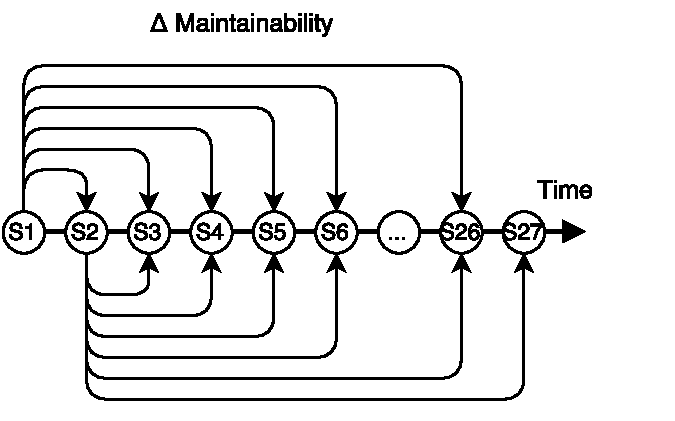
\includegraphics[width=0.50\textwidth]{figs/extraction.pdf}
  \caption{State transition extraction schema for first two snapshots. Circles denote snapshots. Every arrow connecting two snapshots denotes an extracted transition.}
\end{figure}

To investigate the change of maintainability, each snapshots was extracted together with maximum 25 proceeding snapshots belonging to the same system. With a given median snapshot distance of 7 days and an average of 13 snapshots per system we expect that this set of snapshots cover at least a time span of 13 weeks for most systems. Then, for each series, maintainability deltas and time deltas between first and n-th proceeding snapshot were determined. Every transition was saved together with information about it's start state and it's end state. Code change related metrics were commulated over all snapshots between start and end. Figure 1 visualizes this extraction process and Table \ref{data_points} shows the resulting extracted features.
\begin{table}[htbp!]
\caption{Attributes of Extracted Transition Data Points}
\begin{tabular}{l  p{5.2cm}}
  \hline			
  Property & Description \\ \hline
  Snapshot ID & ID of start snapshot \\
  Maintainability & Maintainability of start snapshot\\ 
  Volume & Volume of start snapshot\\ 
  Maintainability delta & \(\Delta\)(Maintainability start, Maintainability end)\\
  Time delta & \(\Delta\)(Date start, Date end)\\
  LOC start & Total lines of code of start snapshot\\ 
  LOC end & Total lines of code of end snapshot\\ 
  Changed lines & Commulative changed lines between start and end snapshot \\
  Code Churn & Commulative code churn between start and end snapshot \\ 
  Deleted lines & Commulative deleted lines between start and end snapshot \\ \hline
\end{tabular}
\label{data_points}
\end{table}

After excluding transitions which do not show any code changes $\sim$300000 data points were left for the following analysis.

\subsection{Maintainability Change Base Rate}

\subsection{System Grouping}
We preferred using cluster center as starting point for the grouping process instead of an equally spaced grid on the data. This gives us the advantage of groups which have small inner-group and large between-group variances.
The number of cluster was chosen to be 125, which is approximately the number of all combinations of maintainability and volume in 0.5 point steps and is as well in line with the Kanti's rule of thumb \cite{kanti1979multivariate} of \(k\approx\sqrt{50000/2}\approx158\). 

Clustering was performed with Weka~\cite{hall2009weka} using k-means clustering with Euclidean distances based on maintainability and volume.
Due to the correlation between maintainability and volume, not every combination of volume and maintainability is equally supported by data. This does though not lead to substantial problems for later analysis.

Subgroups of systems were built around the cluster center, by selecting the 5\% closest (Euclidean distance) data points to each cluster center. This leads to 125 subgroups of \textasciitilde15000 elements each. It is to note that same data points can be assigned to multiple subgroups if they are lying close to each other. The groups are not disjoint on purpose, in that way each subgroups can contain a larger amount of data points which will be essential for getting stable quantile estimation in the next step. The resulting group center are additionally not significantly different from the previously determined cluster center.

\subsection{Maintainability/Volume Aware Change Rate}
Maintainability change was analyzed for each of the previously determined groups separately, over time, leading to a plot as in Figure 2. The dark points mark the weekly 10th and 90th percentiles and the red lines are quantile regression lines on the same percentiles. The upper red line marks the maintainability improvement of the 'top-performers' and the lower line the deterioration of the 'worst-performer'. The plot shows data for the first 13 weeks only, while the quantile regression line was fitted on the full data set which contains support for up to 26 weeks to over-fitting on the 13 week interval. Two different quantile regression models were fitted to the data: \(percentile\sim sqrt(time)\) and \(percentile\sim sqrt(time)+time\). Both lead to comparable sum of squared error rates over all systems, but the latter model was chosen because of the additional linear term, which creates more realistic fits corner cases in which the change rate is very low or changes direction. 
The cone spanning between top-performer and worst-performer describes the 80\% confidence interval in which a system of that type will end up during the next 13 weeks, based on observations in the given dataset. This can already be considered as a useful approach to benchmark the quality improvement performance of a specific system.
\begin{figure}[htbp!]
  \label{cone}
  \centering
  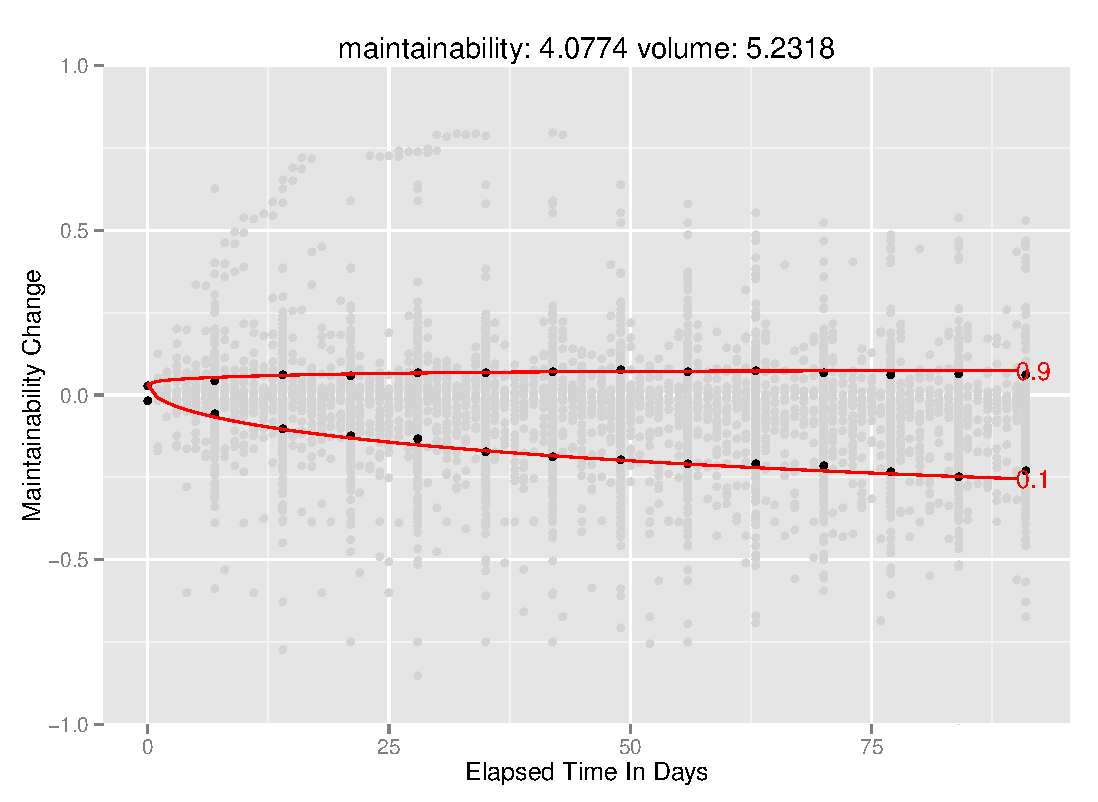
\includegraphics[width=0.5\textwidth]{figs/graph_m_4v_5.pdf}
  \caption{Maintainability change quantile regression (10th and 90th percentile, \(percentile\sim sqrt(time)+time\)) over 13 weeks, for a specific group of systems around cluster center m=4.0774, v=5.2318}
\end{figure}
However, first visual inspection of the resulting plots for each group showed significantly different cones, which leads to the conclusion that hypothesis H1 can be confirmed. Further objective was to explain the difference, by maintainability and volume of the respective groups. 
The ambitions to fit a linear regression model on the quantile regression parameter of the upper and lower line, did not lead to promising results. 
Subsequently, a model was fitted on the upper (90th) and lower (10th) maintainability change percentiles in the 13th week.  
Linear models for the lower quantile leads to high significance and a high R-square value. Thus, the lower boundary for maintainability change in 13 weeks can be expressed with a simple linear model. Same models on the upper quantile lead though to non-significant results. Further analysis explained the weakness of the first approach and revealed a change in trend at \(maintainability*volume>13.5\). 
Subsequently, both regions were analyzed separately, leading to significant models for both regions. We can thus confirm H2 as well. See Table \ref{correlations} for detailed outcomes of the analysis with and without the interaction term. 
\begin{table}[htbp!]
\caption{Correlation Analysis Results}
\begin{tabular}{l  l l p{0.7cm}}
  \hline			
  Percentile & Formula & R-sq. & sign.\\ \hline
  10th & \(perc\sim v+m\) & 0.78 & \textless 0.001\\
  10th & \(perc\sim v+m+v*m\) & 0.92 & \textless 0.001\\ 
  90th (MxV\textless13.5) & \(perc\sim v+m\) & 0.72 & \textless 0.001\\
  90th (MxV\textless13.5) & \(perc\sim v+m+v*m\) & 0.75 & \textless 0.01\\
  90th (MxV\textgreater=13.5) & \(perc\sim v+m\) & 0.77 & \textless 0.001\\
  90th (MxV\textgreater=13.5) & \(perc\sim v+m+v*m\) & 0.82 & \textgreater 0.05\\
\end{tabular}
\label{correlations}
\end{table}

Because of acceptable r-squared values and residual plot for model with and without interaction terms, we decided to present the more intuitive interpretable results for the linear models without interaction terms (see Table \ref{results}).
\begin{table}[htbp!]
\centering
\caption{Linear Regression Models on Upper and Lower Bound for Maintainability Change over 13 Weeks}
\begin{tabular}{l  l  l p{1.2cm}}
  \hline			
  Percentile & Intercept & M & V\\ \hline
  10th & 0.253116 & -0.020066 & -0.085102\\ 
  90th (left) & -0.115953 & 0.039481 & 0.024165\\
  90th (right) & 0.414851 & -0.147388 & 0.056140\\
\end{tabular}
\label{results}
\end{table}

\subsection{Benchmark}
objectivity, reliability, validity.
average quantile in their group
Because objective of this study is not to make a point prediction for one specific system, but to reveal an underlying trend regardless of how one individual projects behaves. One specific system might improve in one week and deteriorate or stay the same in the next week, which depends on various factors which are certainly not completely covered by the current data set. But we hypothesize that maintainability and volume are the two main driving factors for maintainability improvement potential. To measure the improvement potential we want to determine the upper 90\% quantile of maintainability improvement in a subgroup, which is based on maintainability and volume rankings. This would reflect the amount of improvement which the 'top-performer' of certain subgroup achieved and thus implicitly mark an upper bound for improvement of a specific system category. We want to point out that maintainability and volume are not the only possible factors influencing the improvement of maintainability, but the hypotheses give us a starting point to develop a set of methods, which can be used to investigate different factors in future work as well.

%%% Local Variables:
%%% mode: latex
%%% TeX-master: "IWSM-Mensura-2016"
%%% End:
